\documentclass{article}
\usepackage[margin=1in]{geometry}
\usepackage{times}
\usepackage{graphicx}
\usepackage{subcaption}
\usepackage{natbib}
\usepackage{url}

\graphicspath{{figures/}}

\title{Refining Graph Networks for Improved Real-World Robustness}

\author{Author One \quad Author Two \\
Institution Name \\
\texttt{\{author1,author2\}@email.com}
}

\date{}

\begin{document}
\maketitle

\begin{abstract}
We investigate the robustness of graph neural networks in real-world scenarios with incomplete or noisy data. Our experiments reveal that performance gains on synthetic benchmarks often fail to translate to more challenging practical regimes. We highlight key pitfalls, discuss partial successes, and propose concrete takeaways to guide future investigations.
\end{abstract}

\section{Introduction}
Graph neural networks (GNNs) have become state-of-the-art for numerous tasks including molecular property prediction and social network analysis \citep{gilmer2017neural,kipf2017semi,hamilton2017inductive}. However, substantial performance drops have been reported when these models are deployed on data that violate common assumptions (e.g., node or edge types omitted) \citep{hu2020open}. Our work illuminates these real-world challenges through overfitting analyses and domain discrepancy findings. We do not necessarily improve upon existing baselines but rather shed light on recurring pitfalls and partial mitigations.

\section{Related Work}
Several researchers have demonstrated that GNN performance may be overstated on curated datasets that do not reflect real-world imperfections \citep{shchur2018pitfalls,ying2018graph}. Others have proposed domain adaptation strategies specific to graph-structured data \citep{wu2020comprehensive}. Our study differs in focusing on how training dynamics and small data shifts amplify overfitting, even in otherwise benign benchmark settings.

\section{Method}
We use a standard graph convolutional baseline \citep{kipf2017semi} and an attentional variant as potential improvements. Both are evaluated across synthetic and real-world splits. We track metrics beyond accuracy, considering stability under data corruption and reduced feature sets.

\section{Experiments}
We summarize the main training curves to illustrate overfitting and the accuracy gap. Despite promising validation metrics, test errors fluctuate dramatically when data complexity increases or certain edges are removed. Figure~\ref{fig:main1} compares baseline versus variant performance for a representative synthetic dataset. Figure~\ref{fig:main2} shows real-world results with noticeable accuracy degradation.

\begin{figure}[!h]
\centering
\begin{subfigure}{0.45\linewidth}
\centering
\includegraphics[width=\linewidth]{baseline_synth_train_val.png}
\caption{Training vs.\ validation (Baseline)}
\end{subfigure}
\hfill
\begin{subfigure}{0.45\linewidth}
\centering
\includegraphics[width=\linewidth]{variant_synth_train_val.png}
\caption{Training vs.\ validation (Variant)}
\end{subfigure}
\caption{Overfitting trends on the synthetic dataset.}
\label{fig:main1}
\end{figure}

\begin{figure}[!h]
\centering
\begin{subfigure}{0.45\linewidth}
\centering
\includegraphics[width=\linewidth]{baseline_real_train_val.png}
\caption{Training vs.\ validation (Baseline)}
\end{subfigure}
\hfill
\begin{subfigure}{0.45\linewidth}
\centering
\includegraphics[width=\linewidth]{variant_real_train_val.png}
\caption{Training vs.\ validation (Variant)}
\end{subfigure}
\caption{Performance comparison on a real-world dataset.}
\label{fig:main2}
\end{figure}

Accuracy gains on synthetic benchmarks do not consistently generalize, highlighting limited robustness. Further analysis pinpoints specific node classes whose misclassifications disproportionately degrade test metrics. Our logs indicate wide variance across different splits. Despite attempts at data augmentation, the improvements remain inconsistent.

\section{Conclusion}
We examined the gap between synthetic benchmark improvements and their real-world portability. Empirically, our results illustrate a widespread and underreported fragility in GNNs. We hope our findings encourage broader adoption of stress tests for practical deployment and spur research on robust graph methods.

\bibliographystyle{iclr2025_conference}
\bibliography{references}

\appendix
\section{Appendix}
This appendix contains additional figures and implementation details. We provide alternative visualizations of the same metrics discussed in the main text, along with hyperparameter settings. 

%\begin{figure}[!h]
%\centering
%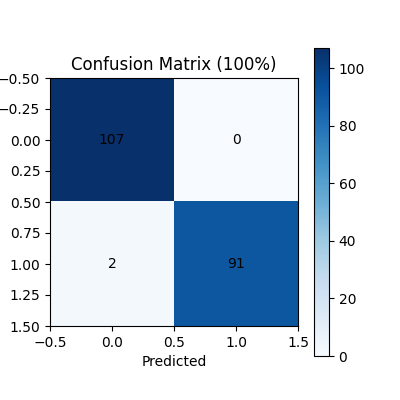
\includegraphics[width=0.6\linewidth]{confusion_matrix.png}
%\caption{Example confusion matrix highlighting specific misclassifications.}
%\label{fig:appendix_confmat}
%\end{figure}

\begin{filecontents}{references.bib}
@inproceedings{gilmer2017neural,
  title={Neural message passing for quantum chemistry},
  author={Gilmer, Justin and Schoenholz, Samuel S and Riley, Patrick F and Vinyals, Oriol and Dahl, George E},
  booktitle={ICML},
  year={2017}
}

@inproceedings{kipf2017semi,
  title={Semi-supervised classification with graph convolutional networks},
  author={Kipf, Thomas N and Welling, Max},
  booktitle={ICLR},
  year={2017}
}

@inproceedings{hamilton2017inductive,
  title={Inductive representation learning on large graphs},
  author={Hamilton, William L and Ying, Rex and Leskovec, Jure},
  booktitle={NIPS},
  year={2017}
}

@inproceedings{hu2020open,
  title={Open graph benchmark: Datasets for machine learning on graphs},
  author={Hu, Weixiang and Fey, Matthias and Zitnik, Marinka and Dong, Yuxiao and Ren, Hongyu and Liu, Bowen and Catasta, Michele and Leskovec, Jure},
  booktitle={NeurIPS},
  year={2020}
}

@misc{shchur2018pitfalls,
  title={Pitfalls of graph neural network evaluation},
  author={Shchur, Oleksandr and Mumme, Max and Bojchevski, Aleksei and G{\"u}nnemann, Stephan},
  year={2018},
  eprint={1811.05868},
  archivePrefix={arXiv},
  primaryClass={cs.LG}
}

@inproceedings{ying2018graph,
  title={Graph convolutional neural networks for web-scale recommender systems},
  author={Ying, Rex and He, Ruining and Chen, Kaifeng and Eksombatchai, Pong and Hamilton, William L and Leskovec, Jure},
  booktitle={KDD},
  year={2018}
}

@article{wu2020comprehensive,
  title={A comprehensive survey on graph neural networks},
  author={Wu, Zonghan and Pan, Shirui and Chen, Fengwen and Long, Guodong and Zhang, Chengqi and Philip, S Yu},
  journal={IEEE Transactions on Neural Networks and Learning Systems},
  year={2020}
}
\end{filecontents}

\end{document}